%
% normal.tex
%
% (c) 2020 Prof Dr Andreas Müller, Hochschule Rapperswil
%
\subsubsection{Vergleich der Fehler}
In diesem Abschnitt vergleichen wir die Fehler der Interpolationspolynome
für die Funktion
\[
f(x)
=
\frac{1}{\sqrt{2\pi}} e^{-x^2/2}
\]
nach Lagrange mit äquidistanten Stützstellen und mit
Tschebyscheff-Stützstellen.

\begin{figure}
\centering
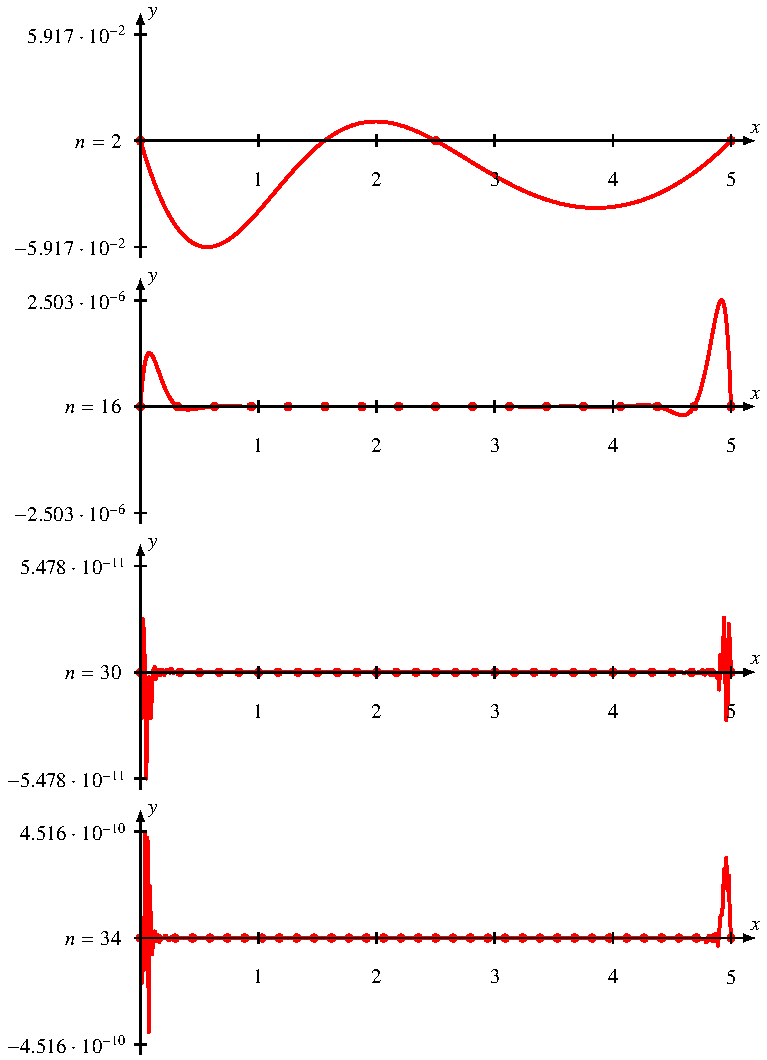
\includegraphics{chapters/30-interpolation/figures/norm.pdf}
\caption{Fehler des Lagrange-Interpolationspolynoms für die Funktion
$f(x)=e^{-x^2/2}/\sqrt{2\pi}$.
Der Fehler nimmt mit der Anzahl der Stützstellen bis $n=30$ ab, danach
wird die Berechnung instabil und der Fehler nimmt wieder zu.
\label{buch:figure:lagrangefehler}}
\end{figure}


\begin{figure}
\centering
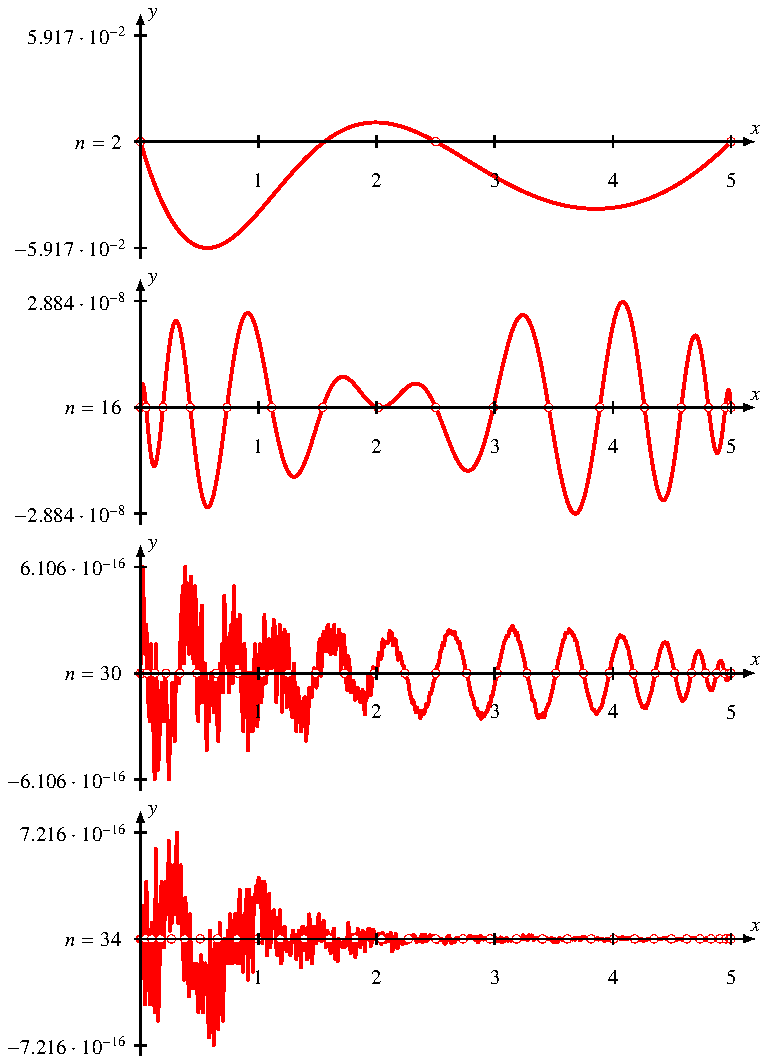
\includegraphics{chapters/30-interpolation/figures/tscheb.pdf}
\caption{Fehler des Interpolationspolynomes für die Funktion
$f(x)=e^{-x^2/2}/\sqrt{2\pi}$ mit Stützstellen nach Tschebyscheff.
Der Fehler bleibt über das ganze Intervall gleichmässig.
Für eine grosse Zahl von Stützstellen erreicht die Interpolation die
Maschienengenauigkeit.
\label{buch:figure:tschebyschefffehler}}
\end{figure}

Die Resultate sind in Abbildung~\ref{buch:figure:lagrangefehler}
für das Lagrange-Interpolationspolynom und
Abbildung~\ref{buch:figure:tschebyschefffehler}
für das Tschebyscheff-Interpolationspolynom
dargestellt.
In beiden Abbildungen wird die gleiche Anzahl Stützstellen verwendet.
Beim Lagrange-Interpolationspolynom nimmt der Fehler zunächst schnell ab.
Er ist, wie das Runge Phänomen erwarten lässt, immer am grössten im
äussersten Teilinterval.
Für grösser werdende Anzahl von Stützstellen wird die Berechnung des 
Interpolationspolynoms in diesen äussersten Teilintervallen instabil
und wächst zum Beispiel von $n=30$ zu $n=34$ um eine Grössenordnung an.
Für eine grosse Zahl von Stützstellen kann das Lagrange-Interpolationspolynom
also mindestens am Rand des Intervalls keine zuverlässigen Approximation sein.

Die Verwendung von Tschebyscheff-Stützstellen verbessert die Genauigkeit
schon bei $n=16$ Stützstellen um zwei Grössenordnungen.
Aussserdem sind die Fehler über das ganze Interval gleichmässig
verteilt.
Bei einer grösseren Anzahl von Stützstellen scheint der Fehler 
vor allem linken Rand stark anzuwachsen.
Da die Funktionswerte aber ungefähr $1$ sind, ist
ein Fehler von $10^{-16}$ genau der typische Rundungsfehler des
\texttt{double} Datentyps.
Man sieht hier als nicht den Fehler des Interpolationspolynoms sondern
die Grenzen der Maschinengenauigkeit.





